\begin{frame}[label=revision-3c]{Respaldo de 3c · Qué operaciones existen en los scripts}
  \small
  \pregunta{¿Dónde están las reducciones que acompañan a cada consulta decimal?}
  \footnotesize
  \begin{tabularx}{\linewidth}{@{}lXXX@{}}
    \toprule Consulta & Dos reducciones principales & Reducción adicional real & Cálculo decimal\\\midrule
    \enlace{q3c1}{3c.1} &
      Totales y menores por departamento: \texttt{map + reduceByKey}. &
      Control nacional: \texttt{values.reduce} sobre totales y menores. \texttt{values} proyecta los valores. &
      \texttt{join + map}: $100\,menores/total$.\\[6pt]
    \enlace{q3c2}{3c.2} &
      Totales y extranjeros por año: \texttt{map + reduceByKey}. &
      Nacionalidades: \texttt{map + reduceByKey} en \texttt{topNacionalidades}. &
      \texttt{join + map}: porcentaje anual.\\[6pt]
    \enlace{q3c3}{3c.3} &
      Totales por mes y total nacional: \texttt{map + reduceByKey}. &
      Trimestres: \texttt{map + reduceByKey} en \texttt{porTrimestre}. &
      \texttt{map}: participación, diferencia e índice.\\
    \bottomrule
  \end{tabularx}
  \begin{block}{Lectura del flujo}
    \footnotesize Cada consulta combina agregaciones principales con una reducción de control o apoyo.
    Después se calcula la razón decimal usando los agregados.
    Los diagramas distinguen estas ramas del cálculo final: no representan tres reducciones consecutivas del indicador.
  \end{block}
  \fuente{Inspección de code/rdd/03c\_1, 03c\_2 y 03c\_3. Estos diagramas describen operaciones del código, no un conteo medido de jobs físicos de Spark.}
\end{frame}

\begin{frame}[label=captura-pg]{Ítem 4 · Evidencia guardada de PostgreSQL funcionando}
  \centering
  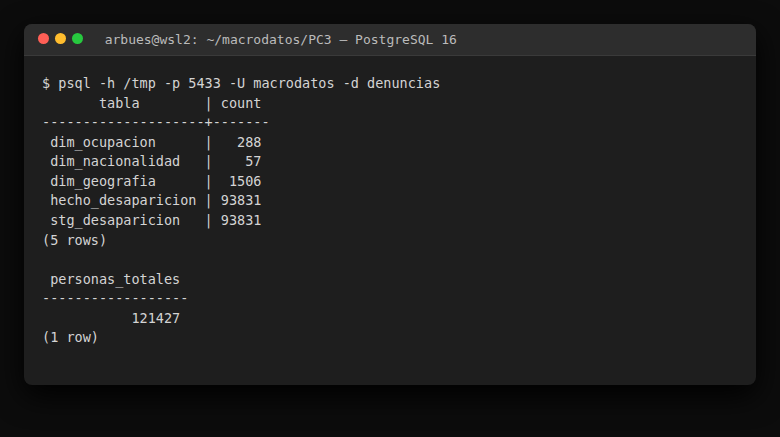
\includegraphics[width=0.94\linewidth,height=5.9cm,keepaspectratio]{../evidencias/pg-conteos.png}
  \fuente{Captura existente: evidencias/pg-conteos.png. Contraste textual: pg-conteos.txt y pg-restauracion.txt.
    \enlace{etl}{Volver al modelo ETL}.}
\end{frame}

\begin{frame}[label=fuentes]{Fuentes, código y reproducción}
  \small
  \begin{itemize}
    \item \textbf{Enunciado:} \texttt{material/L3-cc531-26-2.pdf}, puntos 1--9.
      El punto 7 determina la estructura de cada ficha.
    \item \textbf{Fuente del dataset:} MININTER, \textit{Denuncias por desaparición de personas}. PNDA.\\
      {\scriptsize\url{https://www.datosabiertos.gob.pe/dataset/denuncias-por-desaparici\%C3\%B3n-de-personas-mininter}}
    \item \textbf{Datos locales:} \nolinkurl{data/denuncias_desaparicion_2019_2024.csv}.
    \item \textbf{Código:} \texttt{code/comun/}, \texttt{code/rdd/} y \texttt{code/sql/}.
      Cada ficha importa un fragmento original y referencia la salida guardada.
    \item \textbf{Resultados:} \texttt{evidencias/salidas/}, \texttt{excel/} y \texttt{evidencias/pg-*}.
    \item \textbf{Base de datos:} \texttt{sql/01\_ddl.sql}, \texttt{sql/02\_etl.sql},
      \texttt{sql/dump-denuncias.sql}.
  \end{itemize}
  \begin{block}{Comandos del proyecto para reproducir resultados}
    \footnotesize
    \texttt{./bin/ejecutar.sh code/rdd/03a\_max\_min\_por\_sexo.scala}\\
    \texttt{./bin/correr\_todas.sh}\\
    La ejecución requiere ajustar las rutas absolutas de la instalación original.
  \end{block}
  \fuente{Esta revisión de la presentación usa resultados ya guardados. No vuelve a ejecutar Spark ni PostgreSQL.}
\end{frame}
